% !TEX encoding = UTF-8 Unicode

\documentclass[a4paper]{article}

\usepackage{color}
\usepackage{url}
\usepackage[T2A]{fontenc} % enable Cyrillic fonts
\usepackage[utf8]{inputenc} % make weird characters work
\usepackage{graphicx}
\graphicspath{ {slike/} }
\usepackage{amssymb}


\usepackage[english,serbian]{babel}
%\usepackage[english,serbianc]{babel} %ukljuciti babel sa ovim opcijama, umesto gornjim, ukoliko se koristi cirilica

\usepackage[unicode]{hyperref}
\hypersetup{colorlinks,citecolor=green,filecolor=green,linkcolor=blue,urlcolor=blue}

%\newtheorem{primer}{Пример}[section] %ćirilični primer
\newtheorem{definicija}{Definicija}[section]

\begin{document}

\title{Verifikacija softvera kroz proveravanje modela i simboličko izvršavanje sa alatom KLEE \\ \small{Seminarski rad u okviru kursa\\Metodologija stručnog i naučnog rada\\ Matematički fakultet}}

\author{Ljubica Peleksić, Milica Kojičić \\ peleksic.ljubica@gmail.com, milicakojicic@gmail.com}
\date{31.~mart 2016.}
\maketitle

\abstract{Mnoge klase grešaka je teško naći bez izvršavanja koda deo po deo. Neophodnost takvog testiranja, s obzirom na slabe performanse random i manualnih pristupa, dovela je do iscrpnih radova o drugim značajnim tehnikama verifikacije softvera poput proveravanja modela i korišćenja simboličkog izvršavanja kako bi se automatizovao proces generisanja test primera. Prolazeći kroz teorijske osnove pravljenja modela i konstruisanja osobina koje želimo da proverimo u našem sistemu, objašnjavamo motivaciju koju su imali \textit{Clarke} i \textit{Emmerson} kada su došli do pojma proveravanja modela i kroz jednostavan primer prikazujemo kako on praktično radi. Zatim se fokusiramo na simboličko izvršavanje koje je nezaobilazna alatka za kontrolisanje eksplozije mogućih stanja programa, što je ujedno i najslabija karika proveravanja modela. Pomoću drveta izvršavanja pokazujemo kako se simboličko izvršavanje odvija na primeru, a zatim prikazujemo njegovu osobinu komutativnosti. Dalje se osvrćemo na dokazivanje korektnosti programa pomoću simboličkog izvršavanja. Na kraju prikazujemo alat za simboličko izvršavanje \textit{KLEE}, njegovu upotrebu, način korišćenja, arhitekturu i izuzetnu mogućnost da ga korisnik prilagođava samom sebi.}

\tableofcontents

\newpage

\section{Uvod}
\label{sec:uvod}

Od kada postoje računari i programi, postoje i greške u njima. Programeri posvećuju veliku količinu vremena testiranju i debagovanju onoga što su napisali. Istraživanje je već dugo vremena usmereno ka razvijanju i poboljšavanju metoda za testiranje. Testiranje uspešno identifikuje mnoge značajne greške, a opet veliki broj prođe nezapaženo. Baš zbog toga se teži da se kompjuterski sistemi posmatraju kao matematički objekti i da se korektno ponašanje sistema predstavlja matematičkom logikom, a da se zatim proba dati formalan dokaz da program odgovara svojoj specifikaciji. Problem verifikacije glasi: Za dati program \textit{M} i specifikaciju \textit{h} utvrditi da li ponašanje programa \textit{M} zadovoljava specifikaciju \textit{h}. Problem proveravanja modela je instanca problema verifikacije i oba su matematički problemi. Proveravanje modela je generalan pristup verifikaciji koji ima veliki spektar primena, kao što su ugrađeni sistemi, softversko inženjerstvo i hardverski dizajn. Nije zahtevan za učenje i korišćenje, pa se tako sve više koristi u industriji, tj. koriste ga velike kompanije u njihovom normalnom procesu potvrđivanja kvaliteta. \\ 

Glavni problem proveravanja modela je eksplozija stanja sistema koji se proverava, tj. eksponencijalni porast broja stanja. Da bi se to što manje ispoljavalo, uz proveravanje modela koristimo simboličko izvršavanje da bismo lakše baratali kompleksnim struktura na ulazu i da bi se u što većoj meri iskoristile mogućnosti proveravača modela. Pojam simboličkog izvršavanja programa usko je vezan za pojam normalnog izvršavanja programa. Prednost je ta što jedno simboličko izvršavanje može predstavljati velike, obično beskonačne, klase normalnih izvršavanja. Ono je takođe korisno i u drugim aspektima programske analize, uključujući i generisanje test primera kao i u optimizaciji programa.

\section{Proveravanje modela}
\label{sec:naslov1}

Proveravanje modela je tehnika za formalnu verifikaciju koja je nastala kao rešenje za problem verifikacije konkurentnih programa. Greške u konkurentnosti su teške za nalaženje običnim testiranjem programa zato što se teško reprodukuju. To je automatska tehnika, što znači da stalna interakcija sa korisnikom nije potrebna. \textit{Clarke} i \textit{Emmerson} dolaze do ovog pojma 80-ih godina. Radi se o verifikacionoj tehnici koja izučava sva stanja sistema u maniru grube sile. Slično kao kompjuterski program za šah, softverski alat koji izvodi proveru modela prolazi kroz svaki scenario koji sistem može imati. Ovako se može pokazati da dati model sistema zaista zadovoljava određenu osobinu. Proveravanje modela zahteva precizno i nedvosmisleno definisanje osobina koje treba da se provere. Tipične osobine koje se proveravaju su kvalitativne prirode, kao što su: Da li je generisani rezultat ispravan? Da li sistem može razviti mrtvu petlju? Da li dva konkurentna programa mogu da čekaju jedan drugog i da zaustave ceo sistem? Takođe, mogu se proveravati i vremenske osobine, kao što su: Da li se može desiti mrtva petlja jedan sat nakon resetovanja sistema? Da li se uvek rezultat dobija u prvih 8 minuta rada sistema \cite{principles}? \\

Specifikacija osobina opisuje šta bi sistem trebalo da radi, a šta ne, dok model opisa govori kako se sistem \textit{zaista ponaša}. Proveravač modela istražuje sva stanja sistema da bi proverio da li ona zadovoljavaju određenu osobinu. Ako se pojavi stanje koje je u suprotnosti sa osobinom koja se proverava, proveravač modela pravi tzv. \textit{kontraprimer} koji pokazuje kako se došlo do tog stanja, tj. prikazuje putanju od inicijalnog do problematičnog stanja. Uz pomoć simulatora, korisnik može da ponovi loš scenario i tako dobije korisne informacije za debagovanje, kako bi kasnije mogao da prilagodi model. Postoji mogućnost simulacije pre nego što počne samo proveravanje modela. Simulacija je korisna jer se uklanjanju jednostavnije greške u modelu, a samim tim se smanjuje količina vremena i prostora koja je potrebna za kasniju analizu \cite{principles}.\\ 

Da bi se ovakav problem rešio algoritamski, sam model sistema kao i njegova specifikacija moraju da budu formulisani na nekakvom preciznom matematičkom jeziku -- na jeziku \textit{temporalnih logičkih formula}. I u tom smislu treba proveriti da li neka struktura zadovoljava datu logičku formulu. Ta struktura je najčešće data kao opis na industrijskom jeziku za opisivanje hardvera ili na nekom jeziku specifične namene i ona odgovara  nekom konačnom automatu, odnosno  usmerenom grafu koji se sastoji od čvorova i grana. Čvorovi reprezentuju stanja sistema, a grane odgovaraju prelascima između stanja. Problem proveravanja modela lako je postaviti:
\begin{definicija}
Ako nam je data željena osobina, izražena kao temporalna logička formula p i struktura M sa skupom stanja s, treba utvrditi da li  M,s $\vDash$ p. Ako je struktura M konačna, proveravanje se svodi na pretragu grafa. \\
\end{definicija}

Posmatramo problem dva procesa koji se takmiče za deljeni resurs, tj. oba procesa  ne smeju  da pristupaju resursu u isto vreme (na primer proces A hoće da čita, a proces B da menja resurs, pa ne smemo dozvoliti da rade istovremeno kako proces A ne bi pročitao netačne informacije). Procesi se izvršavaju na jednom procesoru u intervalnom maniru.  Komanda \textit{wait} stavlja proces na spavanje. Kada svi procesi spavaju, planer pokušava da nađe uslov koji zadržava i reaktivira ceo proces. Svaki od procesa ima dva stanja, 0 i 1 i kada je u stanju 1 on pristupa kritičnoj regiji, dok u stanju 0 čeka na drugi proces. Proces može pristupiti deljenom resursu samo dok se nalazi u kritičnoj regiji, što je prikazano na na slici \ref{fig:slika0}.

\begin{figure}[h!]
\begin{center}
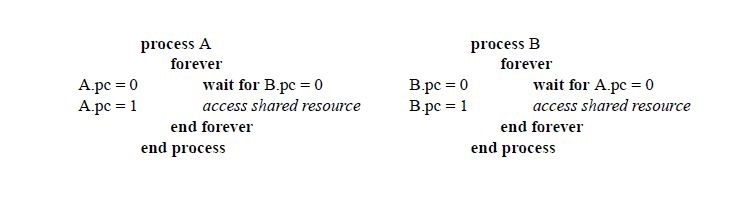
\includegraphics[width=0.95\textwidth]{slika0}
\end{center}
\caption{Prikaz koda dva procesa}
\label{fig:slika0}
\end{figure}

Stanje sistema prikazuju dva brojača, jedan prikazuje stanje procesa A, drugi stanje procesa B. Ono se može kodirati kao binarni vektor dužine 2:
\textit{s $\in$ S = $\lbrace$0,1$\rbrace$ $^{2}$}, gde će prva cifra prikazivati trenutno stanje procesa A, a druga procesa B. Na početku oba brojača imaju vrednost 0, tj. nijedan proces ne 
pristupa kritičnoj regiji, pa se inicijalno stanje \textit{I} prikazuje vektorom 00. Relacija prelaska se sastoji od više
 mogućih prelazaka koji prate sledeća pravila: 
\begin{enumerate}
\item { Ako stanje nije inicijalno, sledeće stanje je inicijalno, 
	tj. ako neki od procesa trenutno pristupa kritičnoj regiji, on mora da izađe iz nje da bi drugi mogao da uđe}
\item { Iz inicijalnog stanja se može preći u 01 ili 10, 
	tj. iz stanja 00 se ne može preći u stanje 11 pošto bi onda oba procesa pristupala kritičnoj regiji, već samo u stanja gde joj jedan od procesa pristupa}
\end{enumerate}
Tako se relacija prelaska \textit{ T $\subseteq$ S$^{2}$ =$\lbrace$0,1$\rbrace$ $^{4}$} može predstaviti kao skup stringova 0100 (iz 01 u 00), 1000 (iz 10 u 00), 1100, 0001, 0010 što je na slici \ref{fig:slika} prikazano granama između čvorova.

\begin{figure}[h!]
\begin{center}
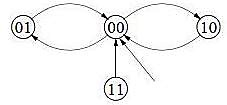
\includegraphics[width=0.7\textwidth]{slika}
\end{center}
\caption{Grafička reprezentacija strukture koja opisuje sistem}
\label{fig:slika}
\end{figure}

Inicijalno stanje ima ulaznu granu bez izvora. Ostale grane predstavljaju ostalih 5 prelazaka. Nedostižno stanje 11 nema ulaznu granu. U njemu se sistem može naći samo ako se iz tog stanja krene, pošto se u njega ne može ući iz nekog drugog. Pošto je inicijalno stanje samo 00, onda se sistem ne može nikako naći u stanju 11 i ono može biti ukolonjeno nakon što se analizom utvrde sva dostižna stanja. Sekvenca 11, 00, 10... je validna putanja ove strukture, ali nije inicijalizovana. Inicijalizovane putanje počinju sa 00, pa je 00, 01, 00, 10... validna inicijalizovana putanja strukture. 
Ovaj primer je siguran zato što samo jedan proces može biti u kritičnoj regiji. Stanje u kome su oba procesa u kritičnoj regiji je nedostižno. Ako bismo dodali granu od 10 ka 11, pretragom u dubinu od početnog stanja 00 kroz stanje 10 došli bismo u stanje 11 i time bi se pokazalo da je loše stanje dostižno i tako bi bezbednosna osobina bila netačna. Ova putanja predstavlja \textit{kontraprimer} koji pomaže da se sistem debaguje \cite{boundedMC}.  \\

Ne postoji nešto što je \textit{korektan sistem} zato što je jedino moguće proveriti da li sistem zadovoljava specifikaciju ili ne. Čak i najnapredniji proveravači modela nisu u mogućnosti da potvrde sve željene oosbine sistema u razumnoj količini vremena, s obzirom na to da za iole složeniji sistem imamo ogroman broj stanja. Proveravači modela se koriste za nalaženje \textit{logičkih grešaka}, a ne za dokazivanje da one ne postoje \cite{boundedMC}. Oni se smatraju dodatnim alatom za ostale tradicionalne metode testiranja i simulacije, a ne alternativnim. Takođe su u mogućnosti da nađu greške koje se verovatno ne bi našle simulatorima, zato što proveravači modela razmatraju sva moguća ponašanja ili izvršavanja sistema. \\ 

Jedna od mogućih alternativa jeste kombinovanje proveravanja modela sa simboličkim izvršavanjem o čemu će biti reč u nastavku. Pošto je priroda podataka kojima program barata takva da je jako teško napraviti model u obliku konačnog automata koji bi predstavio stanje sistema bez ogromne eksplozije stanja, izračunavanja u programu se simbolički modeluju. Naime, smatramo da su u našem modelu ulazne vrednosti predstavljene u obliku vektora simboličkih konstanti $\alpha_i$, dok su numeričke operacije u programu zamenjene odgovarajućim simboličkim operacijama u modelu, što značajno smanjuje broj mogućih stanja i olakšava izražavanje modela u jeziku standardnih alata za proveru modela. Dakle, glavni problem proveravača modela jeste eksplozija stanja i vrlo često se zahteva zatvoren sistem, tj. sistem sa ograničenim okruženjem i ulaznim vrednostima, a ovime mu je baš to i omogućeno. Razni programi mogu na ulazu imati različite kompleksne strukture podataka iz praktično neograničenog domena, pa će se, koristeći simboličko izvršavanje, proveravač modela lakše boriti sa eksplozijom stanja. 
 

\section{Simboličko izvršavanje}
\label{sec:naslov2}
Dalje ćemo se baviti simboličkim izvršavanjem programa. Radi se o tome da se umesto prosleđivanja normalnog ulaza programu, prosleđuju proizvoljne simboličke vrednosti. Izvršavanje programa se odvija normalno, osim što vrednosti mogu biti proizvoljne formule sastavljene od ulaznih simbola. Teški, ali i zanimljivi problemi koji nastaju pri simboličkom izvršavanju, potiču od uslovnih grananja.\\

Testiranje programa i dokazivanje korektnosti programa mogu se posmatrati kao ekstremne alternative. Dok testira, programer pažljivim proučavanjem rezultata može biti siguran da za neki test primer program radi tačno. Tačnost izvršavanja za ulaze koji nisu provereni je i dalje podložna sumnji. S druge strane, pri dokazivanju korektnosti programa, programer formalno dokazuje da program pri svakom izvršavanju ispunjava zahteve koji su dati specifikacijom, a da pritom ne mora da izvršava program uopšte. Da bi to mogao, on daje preciznu specifikaciju tačnog ponašanja programa i dalje sledi formalnu proceduru dokazivanja da bi pokazao da su program i specifikacija konzistentni. Poverenje u ovaj metod zavisi od tačnosti pri kreiranju specifikacije i konstrukcije koraka u dokazu, kao i od mašinski zavisnih problema kao što su prekoračenje, zaokruživanje itd. Ovde se, s druge strane, radi o praktičnom pristupu između ove dve krajnosti. Iz najprostijeg ugla, ovo je poboljšana vrsta tehnike testiranja. Umesto izvršavanja programa nad skupom ulaza, program se \textit{simbolički} izvršava nad klasama ulaza. To znači da rezultat simboličkog izvršavanja može biti ekvivalentan velikom broju uobičajenih test primera. I ovi rezultati svakako mogu biti provereni od strane programera. Klasa ulaza, okarakterisana svakim simboličkim izvršavanjem, određena je u zavisnosti od kontrole toka programa nad ulazom. Ako je kontrola toka programa u potpunosti nezavisna od ulaznih varijabli, jedno simboličko izvršavanje će biti dovoljno da proveri sva moguća izvršavanja programa. Ako pak, kontrola toka zavisi od ulaza, mora se pribeći analizi slučajeva. Često je skup ulaznih klasa koje pokrivaju sve moguće slučajeve beskonačan, tako da je ovo i dalje metoda testiranja. Kako god, ulazne klase su određene samo onim ulazima koji utiču na kontrolu toka i simboličko testiranje obećava postizanje boljih rezultata mnogo lakše od običnog testiranja \cite{simbExec}.\\

U nastavku ćemo se baviti simboličkim izvršavanjem u idealnom smislu, idealnom iz sledećih razloga:
Pretpostavka je da programi obrađuju samo cele brojeve proizvoljne veličine. Drveta izvršavanja koji su rezultat simboličkog izvršavanja su za većinu programa beskonačna. Takođe, simboličko izvršavanje \textit{IF} naredbe zahteva dokazivanje teorema, što je za jednostavnije programske jezike praktično nemoguće ostvariti. Ovaj idealni sistem nam predstavlja standard u odnosu na koji se sistemi za simboličko izvršavanje mogu meriti. Svaki programski jezik ima svoju semantiku izvršavanja, koja opisuje kakve podatke varijable mogu da reprezentuju, kako naredbe manipulišu tim podacima i kojim se tokom odvija izvršavanje naredbi. Paralelno se može definisati alternativna semantika simboličkog izvršavanja, u kojoj se pravi podaci ne koriste, ali mogu biti predstavljeni proizvoljnim simbolima. Simboličko izvršavanje predstavlja prirodnu ekstenziju normalnog izvršavanja, u kojoj su operatori programskog jezika prošireni tako da prihvataju simboličke ulaze i proizvode simboličke formule na izlazu. Pritom, semantika izvršavanja je promenjena u smislu da podržava simboličko izvršavanje, ali ni sintaksa jezika, ni pojedinačni programi pisani u tom jeziku nisu promenjeni. \\
 
Jedini način da se simbolički podaci predstave programu jeste da mu se daju kao ulaz. Svaki put kada program zahteva novu ulaznu vrednost, ona mu se obezbeđuje iz liste simbola \{$\alpha_1, \alpha_2, \alpha_3, ... $ \}. Oni će u nekom trenutku biti dodeljeni kao vrednosti programskim varijablama (kao parametri procedura, globalne varijable i slično). Da bismo mogli da baratamo simboličkim ulazima, dozvoljeno je da vrednosti varijabli mogu da budu $\alpha_i$, kao i celobrojne konstante. I aritmetički izrazi, kao i \textit{IF} naredbe moraju biti proširene tako da mogu da barataju sa simboličkim vrednostima. Time što dozvoljavamo da varijable uzimaju vrednosti polinoma nad $\alpha_i$, simboličko izvršavanje naredbi dodele teče prirodno.
Stanje izvršavanja programa obično uključuje vrednosti varijabli, kao i brojač instrukcija, koji nam daje informaciju o tome koja se naredba trenutno izvršava. Definicija simboličkog izvršavanja \textit{IF} naredbe zahteva da se u stanje izvršavanja uključi i uslov putanje (eng.~{\em path condition - pc}). \textit{Pc} predstavlja logički izraz nad simboličkim ulazima \{$\alpha_i$\}. On nikad ne sadrži programske varijable i možemo ga predstaviti u obliku konjunkcije izraza forme $R \ge 0$ ili  $\neg(R \ge 0)$, gde je \textit{R} polinom nad \{$\alpha_i$\}, na primer:  \{$\alpha_1 > 0 \wedge  \alpha_2 + 3 > 0 $\}. Kao što ćemo videti,  \textit{pc} predstavlja akumulator osobina koje ulaz mora da zadovolji da bi izvršavanje pratilo određenu pridruženu putanju. Svako simboličko izvršavanje počinje tako što se \textit{pc} inicijalizuje na tačno. Kako se prave pretpostavke o ulazima, u cilju odabira putanje koja je određena \textit{IF} naredbom, te pretpostavke se dodaju u \textit{pc}. Simboličko izvršavanje \textit{IF} naredbe teče kao njeno normalno izvršavanje, evaluacijom njoj pridruženog logičkog izraza zamenjivanjem varijabli njihovim vrednostima. Kako su vrednosti varijabli polinomi nad \{$\alpha_i$\}, uslovni izraz je u formi $R \ge 0$, gde je \textit{R} polinom. Nazovimo taj izraz \textit{q}. Koristeći trenutni \textit{pc}, formiramo sledeće izraze: 

\begin{enumerate}
	\item {$pc \supset q$}
	\item {$pc \supset \neg q $}
\end{enumerate}

Najviše jedan od ova dva tvrđenja može biti tačan (eliminišemo trivijalan slučaj kad je \textit{pc} netačan). Kada je tačan jedan od ova dva izraza, nastavlja se sa izvršavanjem \textit{IF} naredbe tako što se kontrola toka prebacuje na njen \textit{THEN} deo ako je izraz (1) tačan ili na njen \textit{ELSE} deo ako je (2) tačno. Ovakav tip izvršavanja se zove neračvajući, jer se izvršava tačno jedna od dve grane, za razliku od slučaja kada ni slučaj (1) ni slučaj (2) nisu tačni. U ovakvoj situaciji postoji skup ulaza u program koji zadovoljava \textit{pc} i koji bi pratio \textit{THEN} alternativu, ali postoji i skup ulaza koji bi išao \textit{ELSE} alternativom. Pošto su obe alternative moguće, jedini kompletan pristup bi bio da se ispitaju obe putanje, tako da se ovde simboličko izvršavanje ''račva'' u dve putanje. Biranjem \textit{THEN} alternative, pretpostavlja se da ulazi zadovoljavaju \textit{q}, pa je ta informacija dodata u \textit{pc}: $ pc \gets pc \wedge q $. Isto tako, biranjem \textit{ELSE} alternative dobijamo $ pc \gets pc \wedge \neg q $. \textit{Pc} se zove \textit{uslov putanje} jer predstavlja akumulaciju uslova koji određuju jedinstvenu kontrolu toka u programu.

\subsection{Drvo izvršavanja}
\label{subsec:podnaslov1}
Drvo izvršavanja opisuje putanje kojima je teklo simboličko izvršavanje programa. Svakom čvoru drveta je priključena izvršena naredba (označena brojem), dok svaka grana između čvorova predstavlja direktnu vezu između naredbi. Za svako račvajuće izvršavanje \textit{IF} naredbe od odgovarajućeg čvora polaze dve veze koje su označene sa \textit{T} i \textit{F} za tačan (\textit{THEN}) i netačan (\textit{ELSE}) deo, respektivno. Takođe se svakom čvoru pridružuju vrednosti varijabli, brojač instrukcija, kao i \textit {pc}. Simbolička izvršavanja za funkciju koja izračunava stepen broja su data na slici \ref{fig:slika2}. Drveta formirana na ovaj način imaju zanimljivu osobinu da za svaki terminalni čvor (koji odgovara kompletno izvršenoj putanji) u drvetu postoji odgovarajući nesimbolički ulaz u program, koji će tokom normalnog izvršavanja programa pratiti istu putanju (listu izvršenih naredbi).

\begin{figure}[h!]
\begin{center}
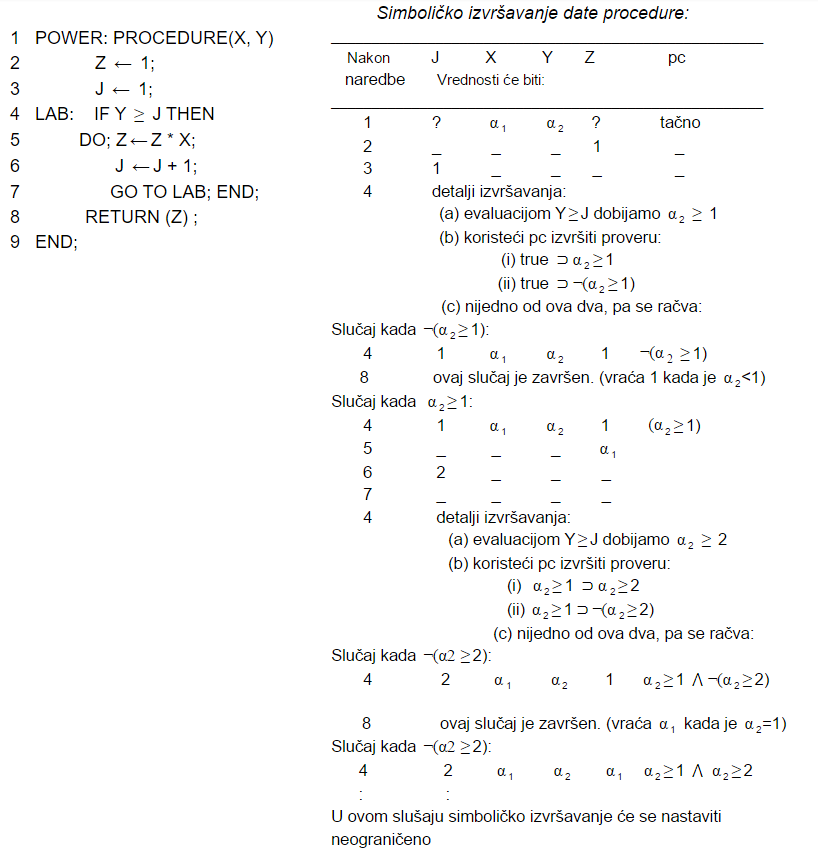
\includegraphics[width=0.7\textwidth]{slika2}
\end{center}
\caption{Simboličko izvršavanje date procedure \cite{simbExec}}
\label{fig:slika2}
\end{figure}


\subsection{Komutativnost}
\label{subsec:podnaslov2}

Ovako definisano simboličko izvršavanje zadovoljava osobinu \textit{komutativnosti}. Naime, ako se program izvršava na konvencionalan način, sa određenim skupom celobrojnih vrednosti \{$j_i$\} na ulazu (dakle prvo se izvrši operacija instanciranja simbola \{$\alpha_i$\} specifičnim celobrojnim vrednostima), rezultat će biti isti ako prvo izvršimo program simbolički, pa onda instanciramo simboličke rezultate (izvršimo dodelu $\alpha_i$=$j_i$). Upravo je ova osobina komutativnosti simboličkog izvršavanja od značaja. Ono proizvodi iste efekte kao i konvencionalno izvršavanje.

\subsection{Simboličko izvršavanje i dokazivanje korektnosti programa}
\label{subsec:podnaslov3}


Pri dokazivanju korektnosti programa, programer uz sam program podrazumeva i \textit{ulazni} i \textit{izlazni} predikat koji  definišu tačno ponašanje programa. Program je korektan ako za sve ulaze koji zadovoljavaju ulazni predikat, rezultati koji proizilaze iz izvršavanja programa (ako ih uopšte ima) zadovoljavaju izlazni predikat. Jedan od koraka pri dokazivanju korektnosti programa - \textit{generisanje uslova verifikacije}, se poprilično lako može uraditi simboličkim izvršavanjem programa. Naime, u testiranju programa (bilo ono simboličko ili ne) moraju da se ispituju izlazi iz programa i mora da se sudi o njihovoj korektnosti.  Ako kriterijum korektnosti može da se formalizuje u smislu ulaznog i izlaznog predikata, onda simbolički izvršilac nakon toga takođe može da pouzdano proveri test rezultate. Za svaki program čije je simboličko drvo konačno i kod koga je kriterijum korektnosti eksplicitno zadat ulaznim i izlaznim predikatima, iscrpno simboličko izvršavanje i dokazivanje korektnosti su zapravo isti proces.


\section{Alat KLEE}
\label{sec:naslov3}

\textit{KLEE} je alat za simboličko izvršavanje, koji može da automatski generiše testove koji postižu veliku pokrivenost na širokom skupu kompleksnih programa. \textit{KLEE} je korišćen za temeljnu proveru 89 samostalnih programa u okviru \textit{GNU COREUTILS}, koji predstavlja jezgro korisničkog okruženja instaliran na milione \textit{UNIX} sistema. Testovi koje je generisao \textit {KLEE} su postigli pokrivenost preko 90\% i značajno prevazišli pokrivenost testova koje su programeri pisali ručno. Takođe, \textit{KLEE} se koristi kao alat za nalaženje bagova i primenjen je na 452 aplikacije (na oko 430K linija koda) gde je našao 56 ozbiljnih bagova, uključujući i 3 u \textit{COREUTILS}-u koji su postojali više od 15 godina. Pored \textit {KLEE}-a, u tabeli \ref{tab:tabela1} su prikazani još neki alati za simboličko izvršavanje. 


\begin{table}[h!]
\begin{center}
\caption{Prikaz različitih alata za simboličko izvršavanje}
\begin{tabular}{|c|c|c|} \hline
\textbf{Alati} & \textbf{Platforma/Jezik}&  \textbf{Otvoren kod} \\ \hline
KLEE& LLVM& Da\\ \hline
Pex& .NET Framework& Ne\\ \hline
JCUTE& Java& Da\\ \hline
Otter& C& Da\\ \hline
Rubyx& Ruby& Ne\\ \hline
\end{tabular}
\label{tab:tabela1}
\end{center}
\end{table}

\textit{KLEE} ima dva cilja: (1) da pokrije svaku liniju izvršnog koda u programu i (2) da detektuje svaku opasnu operaciju (npr. dereferenciranje) ako postoji ijedna ulazna vrednost koja može da prouzrokuje grešku. \textit{KLEE} to radi simbolički, za razliku od normalnog izvršavanja, gde operacije nad operandima proizvode konkretne vrednosti, ovde se generišu ograničenja koja tačno opisuju skup vrednosti koji je moguć na datoj putanji. Kada \textit{KLEE} detektuje grešku ili kada se stigne do \textit{exit} poziva u putanji, \textit{KLEE} rešava ograničenja trenutne putanje (ovo odgovara \textit{pc}-ju spominjanom ranije) kako bi proizveo test primer koji će pratiti istu putanju kada se program ponovo pokrene normalno (kompajlira sa \textit{gcc}). \textit{KLEE} je dizajniran tako da putanja originalnog izvršavanja programa uvek prati istu putanju kojom je išao \textit{KLEE}. Ipak, nedeterminizam u proveri koda i bagovi u samom \textit{KLEE}-u ponekad dovode do toga. \textit{KLEE} koristi različite optimizacije rešavanja ograničenja, reprezentuje stanje programa na kompaktan način i koristi različite heuristike da bi ostvario visoku pokrivenost koda. Takođe, koristi i jednostavan pristup za sinhronizaciju sa okruženjem. Naime, veliki deo koda je kontrolisan vrednostima koje se dobijaju iz okruženja (argumenti komandne linije, fajl sistem). Pošto ulazi mogu biti zlonamerni, program mora biti u stanju da rukuje na pravi način tim ulazima. \cite{klee}.

\subsection{Korišćenje}
\label{subsec:podnaslov1}
Korisnici prvo kompajliraju svoj kod u bajtkod koristeći javno dostupan \textit{LLVM} kompajler za \textit{GNU C}. Pretpostavimo da imamo program 1.c. Kompajliramo ga na sledeći način: 
\[\textbf{llvm-gcc --emit-llvm -c 1.c -o 1.bc}\] 
Dalje se \textit{KLEE} izvršava na ovako generisanom bajtkodu, uz moguće različite opcije koje govore koliko imamo simboličkih ulaza nad kojim testiramo kod, koji je njihov tip i veličina. Za naš program koristimo komandu: 
\[\textbf{klee --max-time 2 --sym-args 1 20 20 1.bc} \]
Prva opcija \textit{--max-time} govori \textit{KLEE}-u da proverava 1.bc najviše dva minuta. Ostatak opisuje simboličke ulaze - opcija \textit{--sym-args 1 20 20} govori da se koristi 0  do 3 argumenta komandne linije, gde se 1. sastoji od jednog  karaktera, a ostala dva od 20. 

\subsection{Arhitektura}
\label{subsec:podnaslov2}
\textit{KLEE} funkcioniše kao hibrid između operativnog sistema za simboličko procesiranje i interpretera. Svaki simbolički proces ima svoje registre, stek, hip, brojač instrukcija i \textit{uslov putanje} - \textit{pc}. Da bismo izbegli konfuziju sa procesima u \textit{UNIX} sistemima, simboličke procese ćemo da nazivamo \textit{stanjima}. Programi se kompajliraju na \textit{LLVM} asemblerski jezik, koji liči na \textit{RISC}  skup instrukcija. \textit{KLEE} direktno interpretira ovaj skup instrukcija i mapira svaku instrukciju u uslov. U svakom trenutku \textit{KLEE} može da izvršava veliki broj stanja. Jezgro \textit{KLEE}-a je interpreterska petlja koja bira stanje koje će da izvrši i dalje simbolički izvršava svaku pojedinačnu instrukciju u kontekstu tog stanja. Ova petlja se izvršava sve dok više nema stanja za izvršavanje ili je korisnički definisano vreme isteklo. Za razliku od normalnih procesa, memorijske lokacije stanja - registri, stek i hip -  referišu na drveta umesto na sirove podatke. Listovi ovih drveta su simboličke promenljive ili konstante, a unutrašnji čvorovi su operacije \textit{LLVM} asemblerskog jezika. \\

Što se instrukcija grananja tiče, tu \textit{KLEE} koristi \textit{STP}, odnosno rešavač ograničenja (eng.~{\em constraint solver}) kako bi utvrdio da li je uslov tačan ili netačan na trenutnoj putanji. Ako jeste, brojač instrukcija se ažurira na odgovarajuću lokaciju, inače su obe grane moguće i tada \textit{KLEE} klonira stanje tako da može da istraži obe putanje. Potencijalno opasne operacije implicitno generišu grane koje proveravaju da li neka od ulaznih vrednosti može da proizvede grešku. Na primer, instrukcija deljenja generiše granu koja proveravala da li je delilac 0. Ako je greška detektovana, \textit{KLEE} generiše test primer koji je hvata i završava to stanje. Problem je što broj stanja u praksi eksponencijalno raste, čak i za najmanje programe \textit{KLEE} generiše na stotine i hiljade stanja tokom nekoliko minuta interpretiranja. Skoro uvek, cena rešavanja ograničenja je dominantna u odnosu na sve ostalo i upravo je ona zaslužna za NP-kompletnu logiku \textit{KLEE}-a i zato se ulaže mnogo truda u pojednostavljivanje izraza pre nego što oni stignu do STP-a \cite{klee}. 


\section{Zaključak}
\label{sec:zakljucak}

Iako ne možemo nikada dati garanciju da je sistem apsolutno korektan, proveravanje modela je tehnologija koja je efikasna u nalaženju grešaka u dizajnu programa i može značajno da podigne nivo poverenja u njega.
Proveravanje modela zajedno sa simboličkim izvršavanjem danas zauzimaju značajno mesto u industriji, gde su aplikacije sigurnosno ili ekonomski bitne. Koriste ih velike kompanije kao što su \textit{IBM, Intel, Microsoft} i \textit{NASA}. Kako napreduje veličina i složenost sistema koje pravimo, proporcionalno raste i broj i obim grešaka. Kako ih ne možemo nalaziti ručno, izuzetno je bitno da razvijamo alate koji će nam pomoći u njihovom nalaženju i prepoznavanju. Glavni cilj je da se u budućnosti za neki proizvoljan program rutinski može pokriti vise od 90\% koda i da se pritom pokriju svi interesantni ulazi. Iako je još uvek dug put ka tome, rezultati pokazuju da ovaj pristup dobro radi za širok skup realnih programa. Mogućnosti za dalja istraživanja su raznovrsne, a verovatno bi se najpre trebalo posvetiti bližem upoznavanju alata KLEE i načinima kako se najbolje može upotrebiti ovaj moćan alat. Na zvaničnoj stranici ovog alata su predložene mogućnosti za unapređenje i pozvani su ljudi da se pridruže i da pošalju svoje ideje.


\addcontentsline{toc}{section}{Literatura}
\appendix
\bibliography{seminarski} 
\bibliographystyle{plain}


\end{document}
